\documentclass[a4paper,10pt]{article}

\usepackage[utf8]{inputenc}
\usepackage[hungarian]{babel}
\usepackage{lmodern}
\usepackage[T1]{fontenc} % < and > signs
\usepackage{listings}
%\usepackage{wrapfig}
\usepackage{graphicx}
%\usepackage{multirow}

\title{Parabánya \\ Operációs rendszerek külön feladat \\ dokumentáció}
\author{Thaler Benedek}
\date{2012. Május}
\begin{document}

%fixed width fonts in listings
\lstset{basicstyle=\ttfamily}

	\maketitle
	
	%\tableofcontents

	\section{Bevezető}
A feladat keretében a kiírásnak \footnote{http://home.mit.bme.hu/~bergmann/edu/ParaBanya.pdf} megfelelően egy programot írtam, mely egy szimulációs feladatot hajt végre, különböző módokon, egy vagy többszálon. A program egy bányát szimulál, melyben állomások között útvonalakon csillék cseréjének segítségével lehet köveket szállítani. A szimuláció feladata, hogy meghatározott csillecserét elvégezzen úgy, hogy a kimenet megfeleljen a felállított helyességi kritériumoknak. A megvalósítás nyelve C++, a párhuzamosítást segítő könyvtár az OpenMP, a felhasznált fejlesztőkörnyezet Eclipse PTP.

	\section{Architektúra}
A szekvenciális és a különböző párhuzamos megoldások összehasonlítása érdekében minden kipróbálandó technika köré (tehát a feladatkiírás szerinti feladatok mentén) egy \emph{solution}t készítettem, melyek a program futása során egymás után hajtódnak végre. A különböző megoldások futtatásához tehát újrafordításra vagy egyéb további konfigurációra nincs szükség. A futás során a program a különböző megoldások futási idejét méri, helyességüket ellenőrzi, majd a gyűjtött adatokat megjeleníti. A program fordítási időben, makró definíciók segítségével konfigurálható, melyek magyarázattal együtt megtalálhatóak a \texttt{constants.h} \footnote{https://github.com/erenon/Paramine/blob/master/src/model/constants.h} fájlban. A konfigurálható értékekre ezen dokumentációban \texttt{DEFINÍCIÓ\_NEVE} formában fogok hivatkozni.

    \subsection{Megoldás lefutási koncepciója}
Minden megoldás először inicializálja a saját bányáját, amin a számításait elvégzi (Ez nem számolandó hozzá a futásidőhöz). Ezután pályánként \\ \texttt{BOGIE\_SWITCH\_COUNT} alkalommal kicserél két csillét (Lane::transport()). A csille cseréje során a pálya IDirectionFactory típusú mezője eldönti, hogy felfelé vagy lefelé szállítson köveket. Ezután a célállomás aktuális kőmennyisége alapján megállapításra kerül a pálya addicionális fogyasztása:

\begin{lstlisting}[language=c]
powerConsumption = log(sqrt(rockAmount / 2));
\end{lstlisting}

Következő lépésben a forrás állomás kőmennyiségét egyel csökkentjük, a célállomásét egyel növeljük. A csere végén az állomásokon tárolt csillék kicserélődnek.
    
    \subsection{Megoldás helyessége}
    
Egy megoldás helyesnek tekinthető akkor, ha a lefutás után a következő feltételek teljesülnek:

\begin{itemize}
    \item Egy állomáson sincs negatív mennyiségű kő
    \item Az állomásokon tárolt kövek összege megegyezik a kiindulási összeggel (\texttt{STATION\_COUNT * ROCK\_AMOUNT})
    \item Minden csille azonosító pontosan egy állomáson van jegyezve
\end{itemize}

Egy megoldás helyessége a pályák egyedi fogyasztásától vagy az állomások egyedi kőmennyiségétől független.
    
	\section{Fordítás és futtatás}
	A project unix(-like) rendszeren a project gyökerében állva a következő parancsokkal fordítható le:

\begin{lstlisting}[language=bash]
parabanya$ cd Debug
parabanya/Debug$ make clean
parabanya/Debug$ make all
\end{lstlisting}

    Ezután a program a következőképpen indítható el a gyökérben állva:
    
\begin{lstlisting}[language=bash]
parabanya/$ ./Debug/parabanya
\end{lstlisting}    	
	
	
	\section{Eredmények}
	Az alábbiakban a megjelölt környezetben elvégzett futási eredményeket és az azokból levont rövid tanulságokat ismertetem, megoldásonként (solution) külön-külön. Minden megoldásnál feltüntetem az inicializáló függvényét, a megoldás helyességét (helyes, helytelen), helytelen megoldás esetén a hibaüzenetet, a futási időt valamint a végállapotot. Felhívom a figyelmet, hogy a feltüntetett futási idők csupán tájékoztató jellegűek, nem szintetikus környezetben végzett, naív mérések eredményei.
	
	\subsection{Futtatókörnyezet és beállítások}
A programot	egy magontként 2.13 GHz-es órajelű Intel Core2 6420 processzorral és 2 GiB 667 MHz-en járó memóriával rendelkező, Ubuntu 12.04 operációs rendszert futtató számítógépen teszteltem. A konfiguráló beállítások a következőek:

\begin{description}
  \item[\texttt{MAX\_THREAD\_COUNT}]: 16
  \item[\texttt{STATION\_COUNT}]: 5
  \item[\texttt{LANE\_COUNT}]: 4
  \item[\texttt{BOGIE\_SWITCH\_COUNT}]: 10000000
  \item[Real]: double
  \item[DirFac]: Random
\end{description}



    \subsection{Triviális szekvenciális megoldás}
\begin{description}
  \item[Inicializáló függvény]: solutionTrivial
  \item[Helyesség]: HELYES
  \item[Futási idő]: 8 másodperc
\end{description}

\begin{lstlisting}
Stations:
#0: {bogie: 0, rock: 99999906.000000}
#1: {bogie: 1, rock: 100000070.000000}
#2: {bogie: 2, rock: 99999978.000000}
#3: {bogie: 3, rock: 100000040.000000}
#4: {bogie: 4, rock: 100000006.000000}

Lanes:
#0: {consume: 88637664.532650}
#1: {consume: 88637667.878526}
#2: {consume: 88637670.721195}
#3: {consume: 88637668.637343}
\end{lstlisting}

A megoldás egy szálon, az elérhető pályákon végigiterálva végzi a cseréket. Láthatóan mozgatja a köveket, amelyek majdnem egyenletesen oszlanak el (a véletlen mozgatási irány miatt). A csillék eredeti sorrendben maradnak, mivel az összes csere száma osztható a visszarendezéshez szükséges cserék számával. Mivel az egyszálúság miatt nincs konkurencia, a triviális implementáció is megfelel a helyességi követelményeknek.



    \subsection{Triviális párhuzamos megoldás}
\begin{description}
  \item[Inicializáló függvény]: solutionTrivialParallel
  \item[Helyesség]: Helytelen, \emph{Total rock amount mismatch, Duplicated bogie id}
  \item[Futási idő]: 6 másodperc
\end{description}

\begin{lstlisting}
Stations:
#0: {bogie: 2, rock: 99999330.000000}
#1: {bogie: 2, rock: 99989986.000000}
#2: {bogie: 2, rock: 100018870.000000}
#3: {bogie: 2, rock: 100020609.000000}
#4: {bogie: 2, rock: 99998110.000000}

Lanes:
#0: {consume: 87586861.221162}
#1: {consume: 88105516.637443}
#2: {consume: 88195135.946234}
#3: {consume: 88199800.418154}
\end{lstlisting}

Ez a megoldás az előző szekvenciális megoldást felhsználva készült, az állomásokon iteráló ciklus fölé az alábbi sort helyezve:

\begin{lstlisting}[language=c]
 #pragma omp parallel for default(none) shared(mine) private(i)
\end{lstlisting}

Az ilyen módon párhuzamosított módszer gyorsabb lefutást eredményez, viszont hibás megoldást ad. A kimenetben megjelenik a duplikált csille hiba, melyet a csillecsere nem atomi végrehajtására lehet visszavezetni, ugyanis így lehetőség van arra, hogy egy szál inkonzisztens állapotot olvasson, és így hajtson végre cserét (valójában két azonos azonosítót cserél ki). Egy ilyen csere során mindig egy azonosító elveszik, egészen addig, amíg csak egy azonosító marad a rendszerben.
Hibás továbbá a kőmennyiségek összege, ez ugyancsak a kontrollálatlan konkurens elérésnek tudható be. 

    \subsection{Párhuzamos megoldás atomi utasításokkal}
\begin{description}
  \item[Inicializáló függvény]: solutionAtomicParallel
  \item[Helyesség]: Helytelen, \emph{Duplicated bogie id}
  \item[Futási idő]: 8 másodperc
\end{description}

\begin{lstlisting}
Stations:
#0: {bogie: 2, rock: 99999890.000000}
#1: {bogie: 2, rock: 100000038.000000}
#2: {bogie: 2, rock: 99999966.000000}
#3: {bogie: 2, rock: 100000002.000000}
#4: {bogie: 2, rock: 100000104.000000}

Lanes:
#0: {consume: 88449489.989032}
#1: {consume: 88600119.867687}
#2: {consume: 88564276.051837}
#3: {consume: 88521544.212820}
\end{lstlisting}

Az előző megoldás "\emph{Total rock amount mismatch}" hibájának javítása végett a kőmennyiség változtatását atomi műveletre cseréltem:

\begin{lstlisting}[language=c]
#pragma omp atomic
rockAmount++;
\end{lstlisting}

Ennek megfelelően az összes kőmennyiség állandó a rendszerben. Az \texttt{\#atomic} konstrukció biztosítja, hogy a védett memóriaterületet (\texttt{rockAmount}) egyszerre csak egy szál írja, még akkor is, ha a memóriaterület írása egy másik helyen is megtörténhet (Itt az \texttt{incrementRockAmount} és \texttt{decrementRockAmount} függvényekben). 
Az atomi műveletek biztosítása erőforrásigényes, ezért a végrehajtási idő a triviális megoldáshoz képest nőtt. Mivel a csillék cseréje továbbra sem szálbiztos, a megoldás helytelen.

    \subsection{Párhuzamos megoldás kritikus szakasszal}
\begin{description}
  \item[Inicializáló függvény]: solutionCriticalParallel
  \item[Helyesség]: Helyes
  \item[Futási idő]: 12 másodperc
\end{description}

\begin{lstlisting}
Stations:
#0: {bogie: 0, rock: 99999796.000000}
#1: {bogie: 2, rock: 100000108.000000}
#2: {bogie: 3, rock: 100000092.000000}
#3: {bogie: 1, rock: 99999960.000000}
#4: {bogie: 4, rock: 100000044.000000}

Lanes:
#0: {consume: 88387424.230874}
#1: {consume: 87671882.698612}
#2: {consume: 88234402.300065}
#3: {consume: 87455366.551025}
\end{lstlisting}

A triviális párhuzamos megoldás mindkét hibáját javítandó, minden utasítás, ami a csillék cseréjét és a kőmennyiség változtatását végzi, egy nagy kritikus szakaszba került:

\begin{lstlisting}[language=c]
#pragma omp critical
{
    // komennyiseg valtoztatasa
    // csillek csereje
}
\end{lstlisting}

Mivel a kritikus szakasz biztosítja, hogy a védett kódrészt egyszerre csak egy szál hajtsa végre, a megoldás megfelel a helyességi követelményeknek. Másfelől viszont a párhuzamosítható utasítások számát radikálisan csökkenti, így a kritikus szakasz fenntartása és a szálak indításának költsége miatt a futási idő jelentősen elmarad a szekvenciális változathoz képest.
A megoldás további hátránya, hogy egy szál feleslegesen zár ki olyan szálakat, amelyek más állomások között dolgoznának.

    \subsection{Párhuzamos megoldás kritikus szakasszal, cirkuláris bányában}
\begin{description}
  \item[Inicializáló függvény]: solutionCriticalParallelCircular
  \item[Helyesség]: Helyes
  \item[Futási idő]: 12 másodperc
\end{description}

\begin{lstlisting}
Stations:
#0: {bogie: 0, rock: 100000168.000000}
#1: {bogie: 4, rock: 100000030.000000}
#2: {bogie: 3, rock: 100000190.000000}
#3: {bogie: 2, rock: 99999640.000000}
#4: {bogie: 1, rock: 99999972.000000}

Lanes:
#0: {consume: 70713583.618279}
#1: {consume: 70766836.014515}
#2: {consume: 70901170.951417}
#3: {consume: 70811218.826839}
#4: {consume: 70578426.608657}
\end{lstlisting}

Az előző megoldáshoz nagyon hasonló megoldás, azzal az eltéréssel, hogy a használt bányában az első és utolsó állomást is összeköti egy pálya. Mivel 5 útvonal van, az egyedi fogyasztások valamivel alacsonyabbak. Az előző megoldás megállapításai itt is igazak.



    \subsection{Párhuzamos megoldás zárakkal}
\begin{description}
  \item[Inicializáló függvény]: solutionLockParallel
  \item[Helyesség]: 
  \item[Futási idő]: 9 másodperc
\end{description}

\begin{lstlisting}
Stations:
#0: {bogie: 3, rock: 99999790.000000}
#1: {bogie: 2, rock: 100000352.000000}
#2: {bogie: 4, rock: 99999804.000000}
#3: {bogie: 1, rock: 100000084.000000}
#4: {bogie: 0, rock: 99999970.000000}

Lanes:
#0: {consume: 88613382.865674}
#1: {consume: 88637411.749353}
#2: {consume: 88535670.157839}
#3: {consume: 88618655.743884}
\end{lstlisting}

Az előző megoldás teljesítményproblémájának javítása végett ez a megoldás kritikus szakasz helyett zárakat használ. Mielőtt egy állomáshoz hozzá akar férni, azt zárolja:

\begin{lstlisting}[language=c]
omp_set_lock(&station.stationLock);
\end{lstlisting}

Ha egy szál két állomás között szeretne csillét cserélni, mindkét állomást zárolja:

\begin{lstlisting}[language=c]
omp_set_lock(&source.stationLock);
omp_set_lock(&target.stationLock);
\end{lstlisting}

Így nem fordulhat elő inkonzisztens konkurens módosítás. A megoldás hibája, hogy amennyiben két szál szeretne ugyanazon a pályán ellentétes irányban szállítani, előfordulhat, hogy mindkettő zárolja az általa választott forrásállomást (tehát két különböző állomást), majd zárolni próbálja a túloldali állomást -- amit a másik szál előzőleg zárolt. Ebben az esetben holtpont (deadlock) alakul ki, amelynek egy lehetséges felderítéséről később olvashatunk. A problémára megoldást jelenthet, ha a csere előtt a pályát is zároljuk:

\begin{lstlisting}[language=c]
omp_set_lock(&laneLock);
omp_set_lock(&source.stationLock);
omp_set_lock(&target.stationLock);
\end{lstlisting}

Így kizárjuk az előbb felmerült holtpont lehetőségét. Egy valamivel jobb lehetőséget a következő megoldás kapcsán ismertetek, ahol nem bizonyult ez a módszer elegendőnek.
A megoldás megfelel a helyességi feltételeknek, futásideje pedig valamivel rövidebb a kritikus szakaszt használókhoz képest, viszont még mindig gyengébben teljesít, mint a szekvenciális megoldás. Ennek oka a szálak nem megfelelő ütemezése, melynek eredményeképpen a végrehajtás egymásra csúszik, és hasonló várakozás jön létre, mint a kritikus szakaszok esetében. Egy lehetséges jobb ütemezést az utolsó megoldásban írok le.

    \subsection{Párhuzamos megoldás zárakkal, cirkuláris bányában}
\begin{description}
  \item[Inicializáló függvény]: solutionLockParallelCircular
  \item[Helyesség]: Helyes
  \item[Futási idő]: 10 másodperc
\end{description}

\begin{lstlisting}
Stations:
#0: {bogie: 4, rock: 100000042.000000}
#1: {bogie: 1, rock: 100000182.000000}
#2: {bogie: 0, rock: 99999628.000000}
#3: {bogie: 3, rock: 99999948.000000}
#4: {bogie: 2, rock: 100000200.000000}

Lanes:
#0: {consume: 70909994.569379}
#1: {consume: 70909149.123353}
#2: {consume: 70910023.785194}
#3: {consume: 70907511.313573}
#4: {consume: 70909711.376597}
\end{lstlisting}

Az előző megoldáshoz nagyon hasonló megoldás, azzal az eltéréssel, hogy a használt bányában az első és utolsó állomást is összeköti egy pálya. Az előbb bemutatott zárolási technikát használva ez itt gondot okoz, feltételezve a következő forgatókönyvet: Legalább annyi szál dolgozik, ahány pálya van. Minden szál zárol egy pályát. Ezután minden szál zárolja a pálya bal végén található állomást. Ezután minden szál megpróbálja zárolni a jobb oldali állomást, amit a szomszédos szál már előzőleg zárolt (annak ez volt a bal oldani), így holtpont alakul ki. A probléma megoldása lehet, ha az állomásokat számokkal látjuk el, és a szálak kötelesek először mindig az alacsonyabb azonosítóval rendelkező állomást zárolni.

\begin{lstlisting}[language=c]
bool lockSourceFirst = source.getId() < target.getId();
LockStation& firstToLock = (lockSourceFirst) ? source : target;
LockStation& secondToLock = (lockSourceFirst) ? target : source;

omp_set_lock(&firstToLock.stationLock);
omp_set_lock(&secondToLock.stationLock);
\end{lstlisting}

Így a fenti példában az utolsó és első állomást összekötő pályán dolgozó szál az első fázisban az első állomást próbálja majd zárolni az utolsó helyett; sikeres zárolás esetén szomszédja, sikertelen esetén ő maga esik ki a következő zárolási fázisból, így a holtpont nem következik be.
A megoldás helyes, de az előzőleg ismertetett okok miatt a futásidő továbbra is elmarad a szekvenciális megoldástól.

    \subsection{Párhuzamos megoldás, fésű ütemezéssel}
\begin{description}
  \item[Inicializáló függvény]: solutionCombParallel
  \item[Helyesség]: Helyes
  \item[Futási idő]: 6 másodperc
\end{description}

\begin{lstlisting}
Stations:
#0: {bogie: 0, rock: 100000212.000000}
#1: {bogie: 1, rock: 100000058.000000}
#2: {bogie: 2, rock: 99999472.000000}
#3: {bogie: 3, rock: 100000486.000000}
#4: {bogie: 4, rock: 99999772.000000}

Lanes:
#0: {consume: 88637667.841901}
#1: {consume: 88637656.091482}
#2: {consume: 88637667.841841}
#3: {consume: 88637674.291713}
\end{lstlisting}

A megoldás a konkurens szálak munkáját úgy ütemezi, hogy olyan útvonalakhoz férjenek hozzá, amelyek nem szomszédosak. Két fázisban dolgozik, az elsőben a páratlan paritású pályákon végez cseréket, a másodikban a párosakon. Ha egy szál nagyon lemarad, az visszafogja a többit az algoritmus közepén található barikádnál (barrier), valamint a lefutás ideje megegyezik a leglassabb szál futási idejével, mivel más szál nem tudja a munkáját átvenni, viszont a megoldás összességében így is a leggyorsabb helyes megoldás az összes közül; nem tartalmaz kritikus szakaszt és nincs szüksége atomi utasításokra vagy zárakra (lock).
    
	\section{Véletlen számok}
A feladatkiírásnak megfelelően a pályáknak véletlenszerűen kell eldönteni, hogy	felfelé vagy lefelé szállítanak követ. Amikor bevezettem a véletlenszerű döntést -- a libc könyvtári \texttt{rand()} függvényét használva -- a párhuzamosítást használó megoldások teljesítménye nagyon leromlott. Ennek az oka a következő; Mivel az említett függvény pszeudorandom számokat generál, szüksége van egy rejtett állapot olvasására és írására, minden egyes hívás során. Az állapotot minden esetben ugyanarról a memóriaterületről olvassa be, ezért a függvény nem újrahívható, így a szálak blokkolódni fognak.
A megoldást a \texttt{rand\_r(\&unsigned int)} függvény jelentette, mely az állapotot tároló memóriaterületet paraméterül kapja, így minden szál szolgáltatni tudja a maga állapotát, elkerülve az egymásra várást.
	
	\section{Holtpont}
A zárakat használó megoldás fejlesztése közben előfordult egy holtpontot (deadlock) okozó szituáció. A holtpont tünete, hogy a várt magas CPU használat helyett a CPU kihasználtság alacsony (a szálak passzívan várnak egymásra), és a program nem terminál.


A debug eszközzel megvizsgált holtpont a mellékelt képeken látható \footnote{A képek megtekinthetőek és letölthetőek olvasható méretben: http://bit.ly/JTP0dH}. A [2] szál forrásállomásának címe \texttt{0x8050098}, míg célállomásának címe \texttt{0x80500b0} (Első és második kép). Ezzel szemben az [1] szál forrásállomása a \texttt{0x80500b0} címen található, a célállomás pedig a \texttt{0x8050098} címen helyezkedik el.

	\begin{figure}[h]
		\begin{center}
			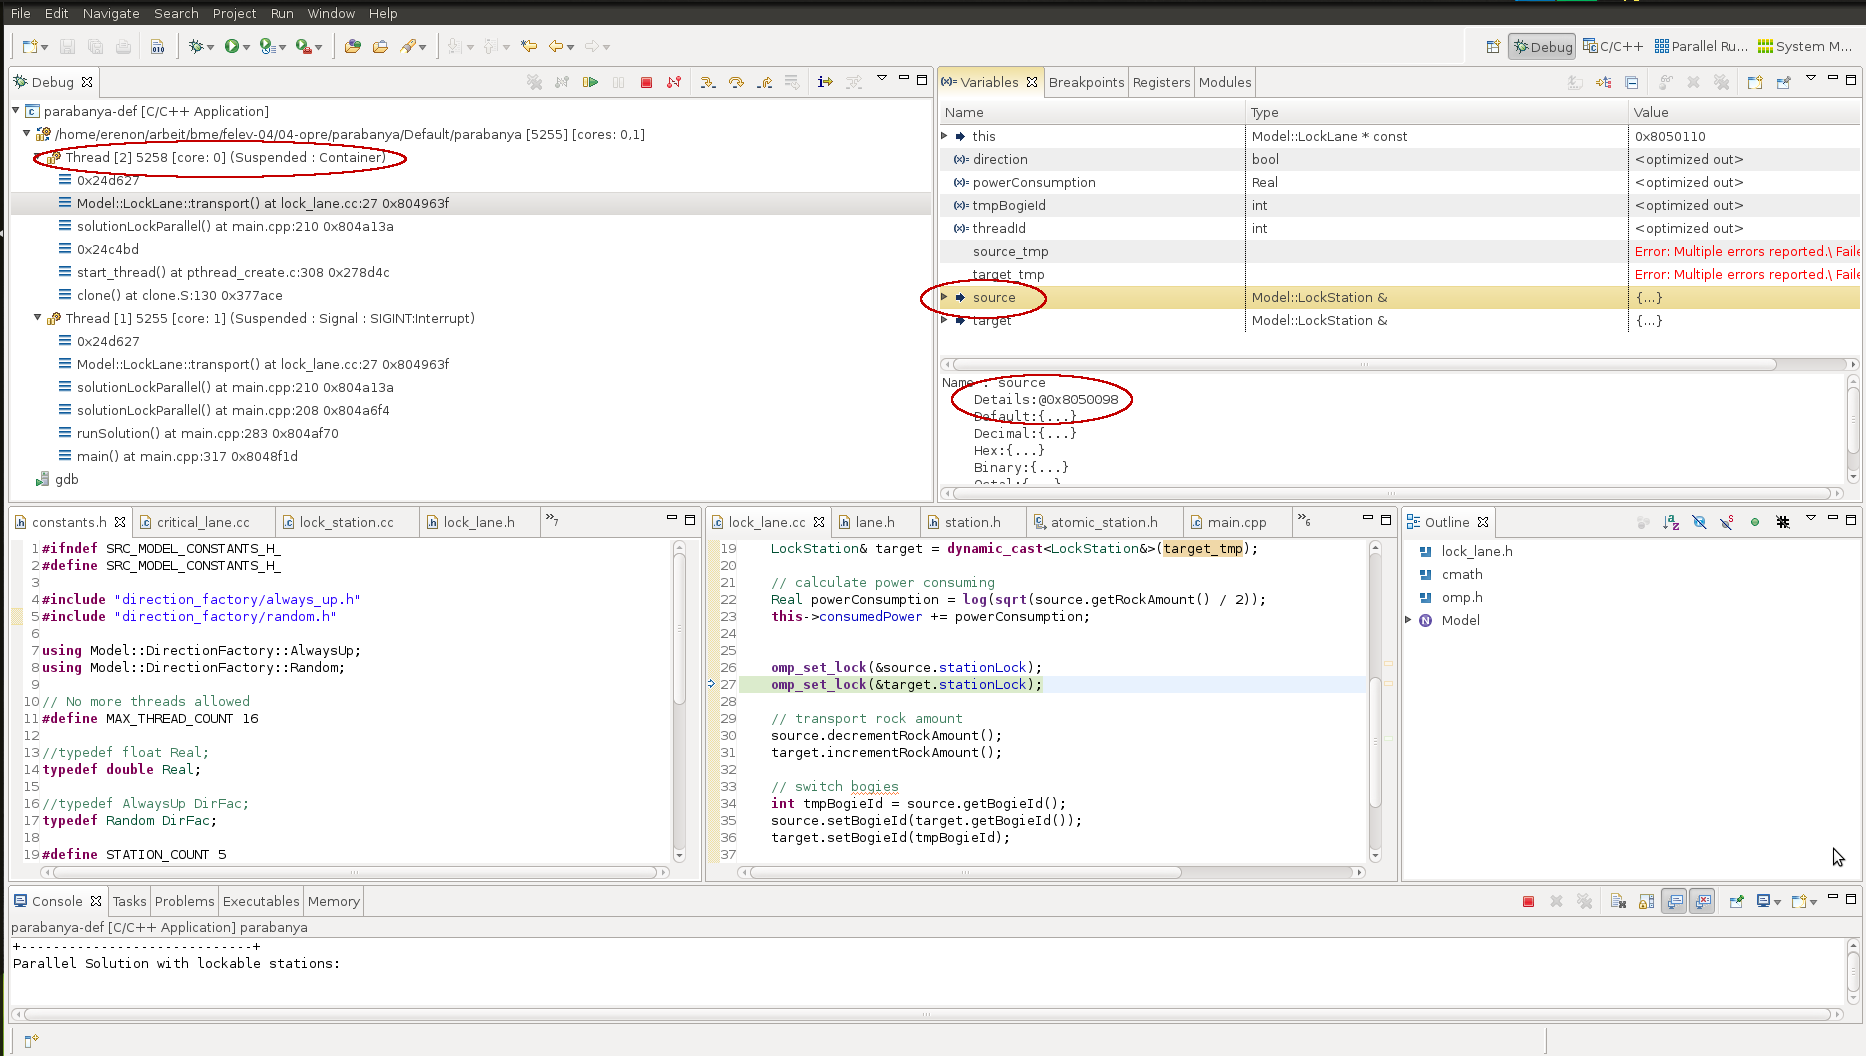
\includegraphics[scale=0.23]{01.png}
			\caption{[2] szál forrásállomásának címe}
		\end{center}
	\end{figure}
	
	\begin{figure}[h]
		\begin{center}
			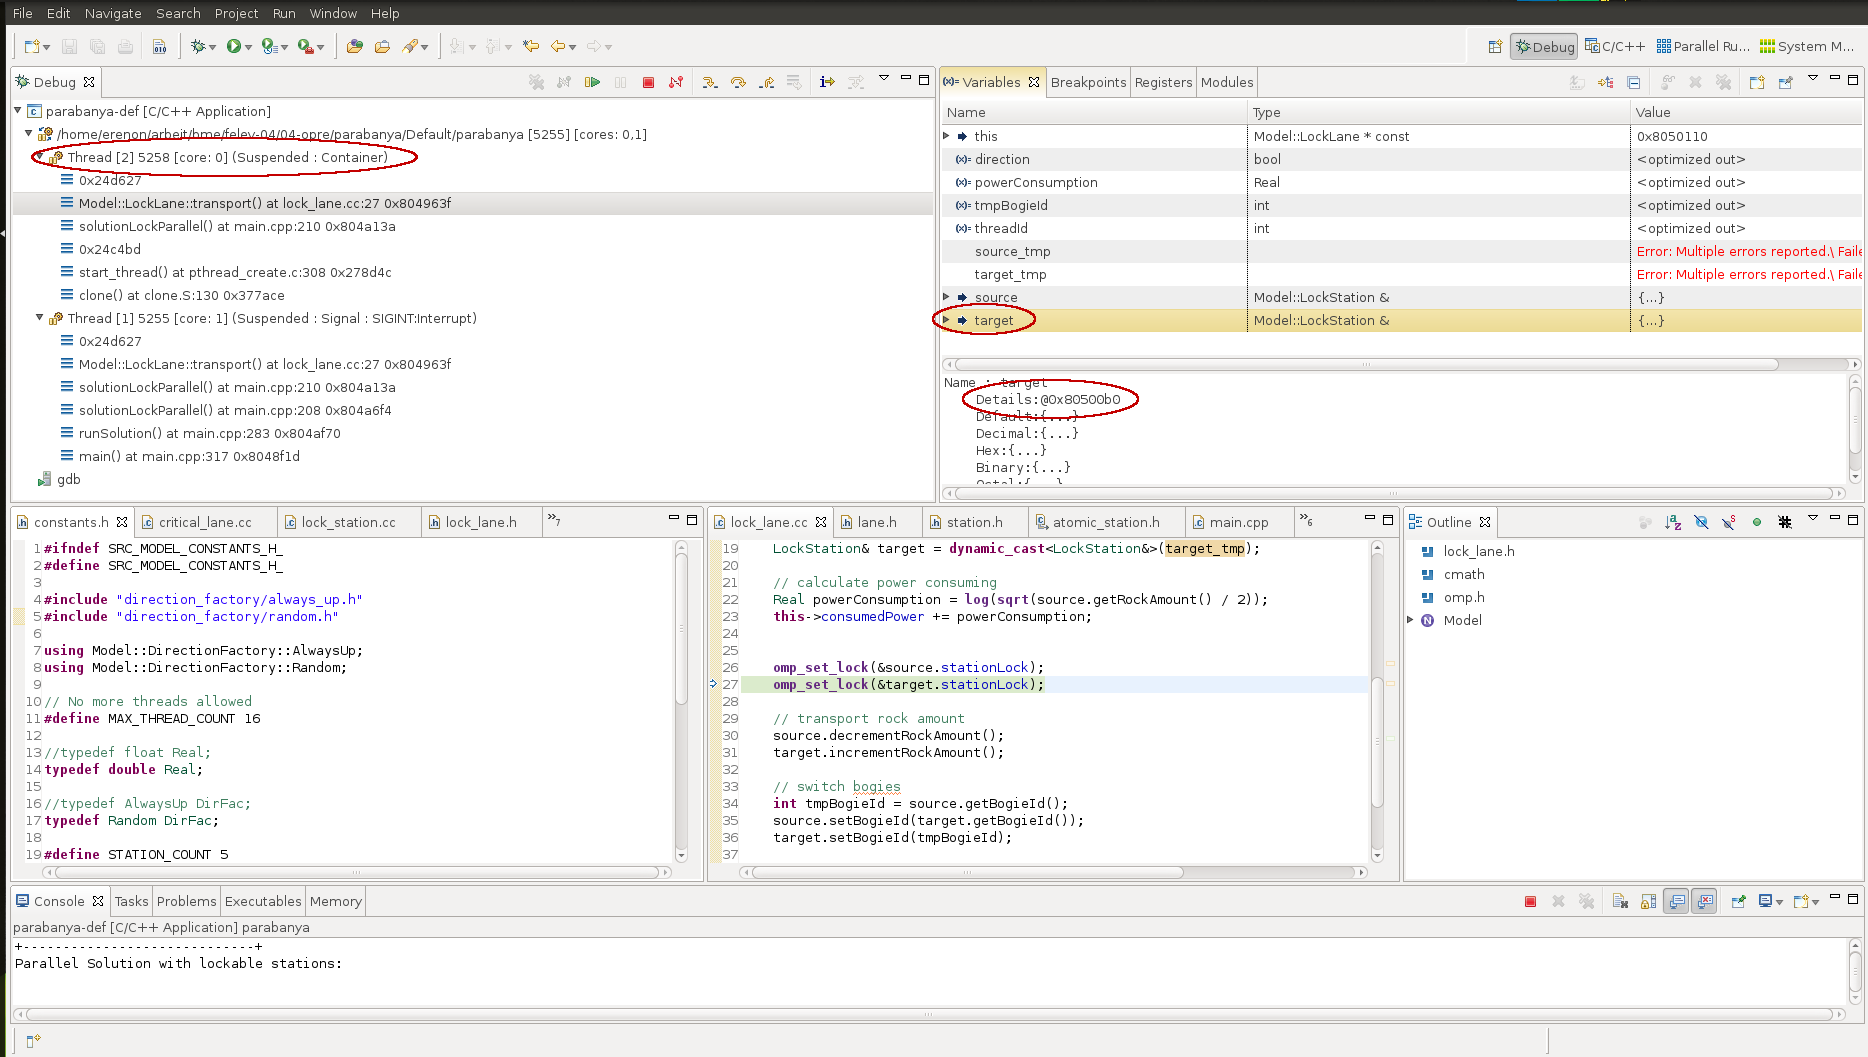
\includegraphics[scale=0.23]{02.png}
			\caption{[2] szál célállomásának címe}
		\end{center}
	\end{figure}
	
	\begin{figure}[h]
		\begin{center}
			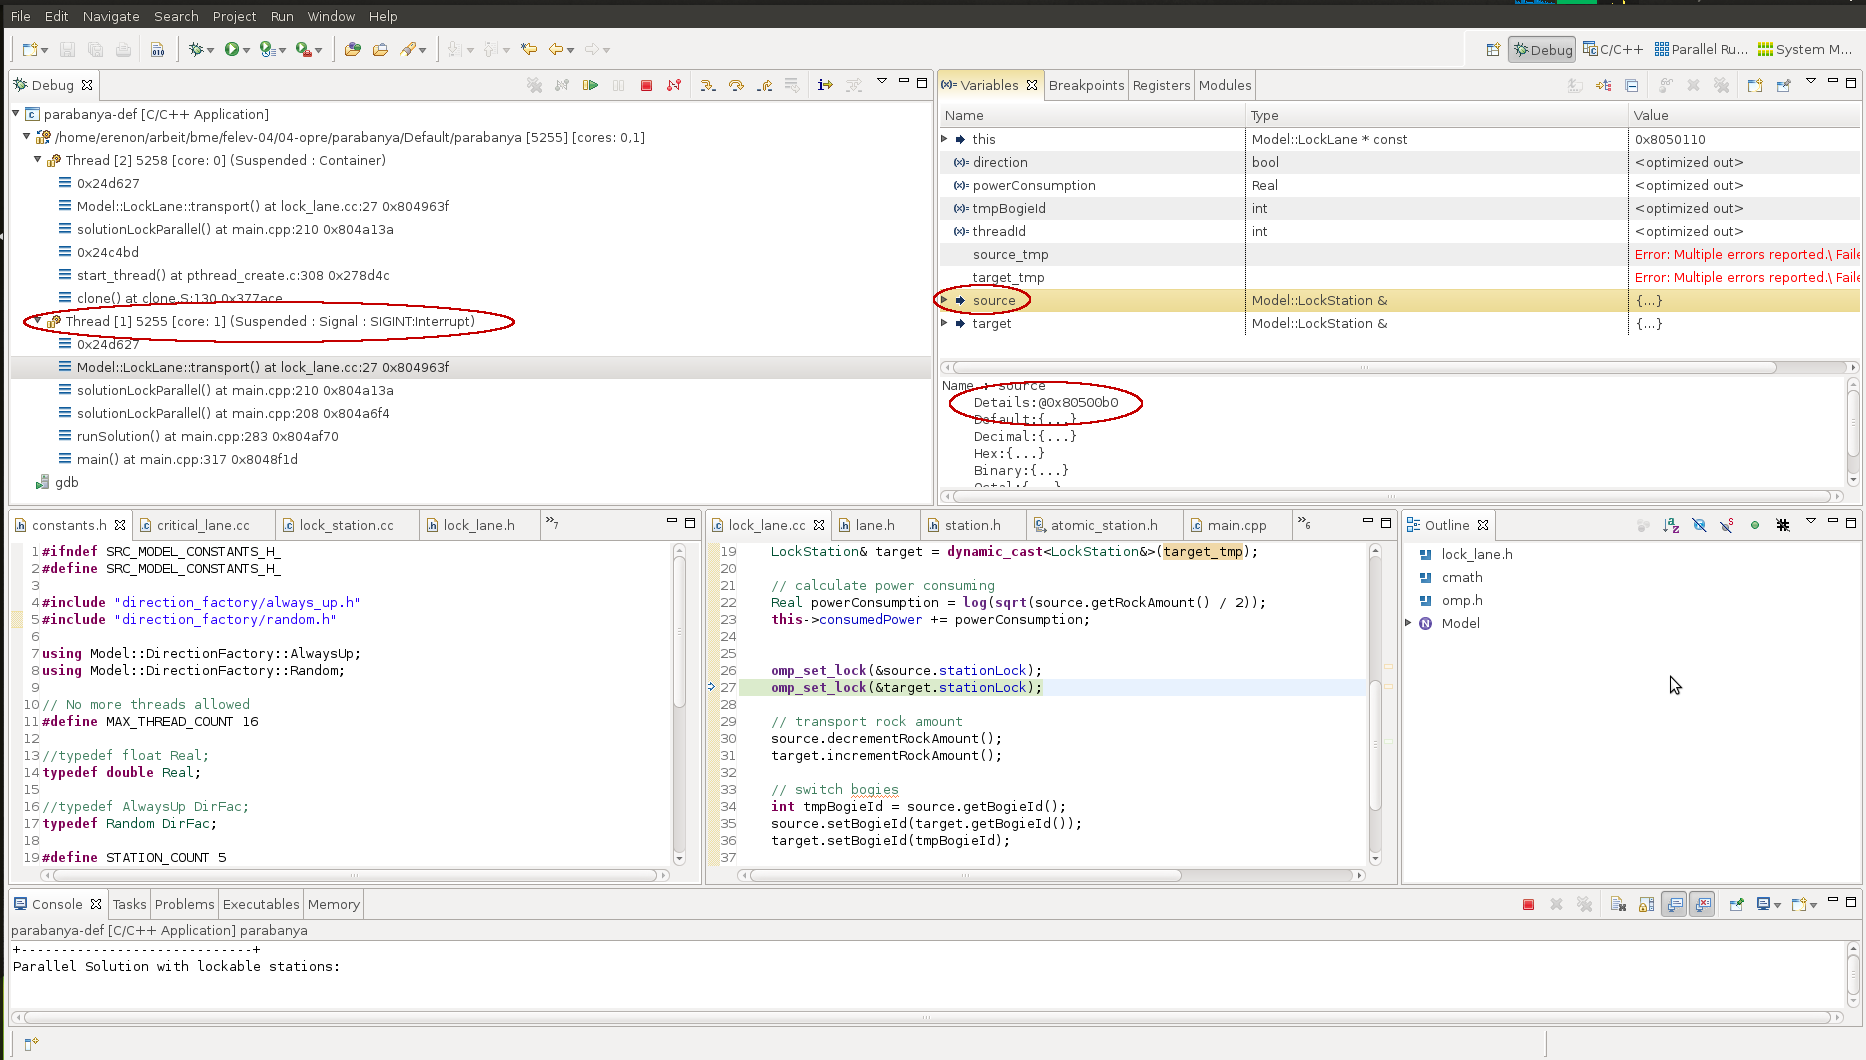
\includegraphics[scale=0.23]{03.png}
			\caption{[1] szál forrásállomásának címe}
		\end{center}
	\end{figure}
	
	\begin{figure}[h]
		\begin{center}
			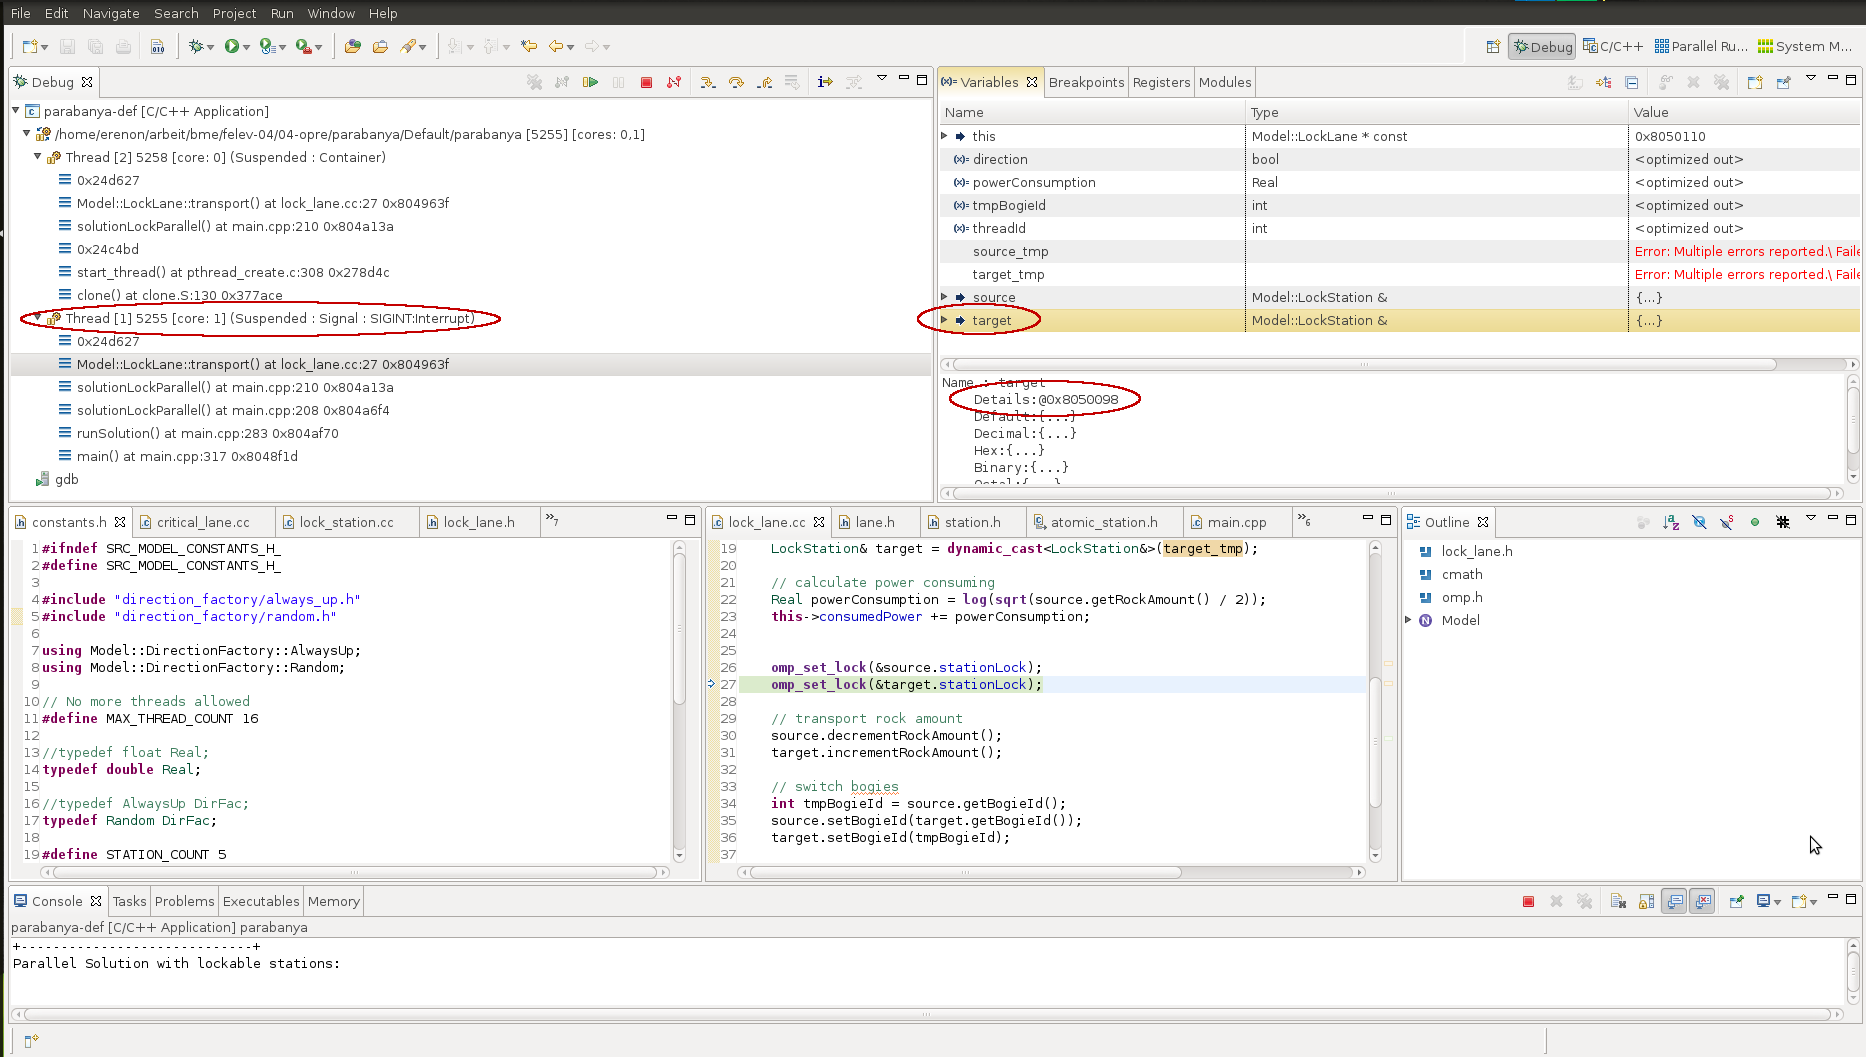
\includegraphics[scale=0.23]{04.png}
			\caption{[1] szál célállomásának címe}
		\end{center}
	\end{figure}

Az aktuális utasítás a második állomás zárolása mindkét szál esetén, viszont azt a zárad mindkét esetben a másik szál már zárolta, így nem tudnak hozzáférni, sem továbbmenni, holtpont alakult ki.

\end{document}
